
\subsection{Breif}
\paragraph{What is Neural Networks?}
Artificial neural networks are one of the main tools used in machine learning. As the “neural” part of their name suggests, they are brain-inspired systems which are intended to replicate the way that we humans learn. Neural networks consist of input and output layers, as well as (in most cases) a hidden layer consisting of units that transform the input into something that the output layer can use. They are excellent tools for finding patterns which are far too complex or numerous for a human programmer to extract and teach the machine to recognize.

\paragraph{}
While neural networks (also called “perceptrons”) have been around since the 1940s, it is only in the last several decades where they have become a major part of artificial intelligence. This is due to the arrival of a technique called “backpropagation,” which allows networks to adjust their hidden layers of neurons in situations where the outcome doesn’t match what the creator is hoping for — like a network designed to recognize dogs, which misidentifies a cat, for example.

\paragraph{}
Another important advance has been the arrival of deep learning neural networks, in which different layers of a multilayer network extract different features until it can recognize what it is looking for.

\subsection{Basics of Neural Networks.}
\paragraph a basic idea of how a deep learning neural network learns, imagine a factory line. After the raw materials (the data set) are input, they are then passed down the conveyer belt, with each subsequent stop or layer extracting a different set of high-level features. If the network is intended to recognize an object, the first layer might analyze the brightness of its pixels.\begin{flushright}
	
\end{flushright}
\begin{figure}{l}
	\centering
	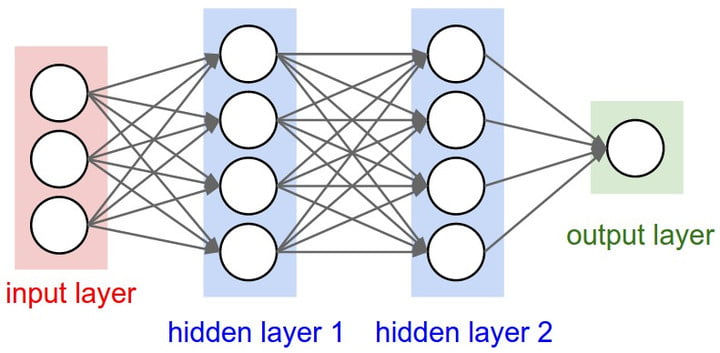
\includegraphics[width=0.5\textwidth]{nn.jpeg}
	\caption{Neural network }
\end{figure}
\paragraph{}
The next layer could then identify any edges in the image, based on lines of similar pixels. After this, another layer may recognize textures and shapes, and so on. By the time the fourth or fifth layer is reached, the deep learning net will have created complex feature detectors. It can figure out that certain image elements (such as a pair of eyes, a nose, and a mouth) are commonly found together.
\paragraph{}
Once this is done, the researchers who have trained the network can give labels to the output, and then use backpropagation to correct any mistakes which have been made. After a while, the network can carry out its own classification tasks without needing humans to help every time.
\paragraph{}
Beyond this, there are different types of learning, such as supervised or unsupervised learning or reinforcement learning, in which the network learns for itself by trying to maximize its score

\subsection{Why Neural networks are important? }
\paragraph{}
ANNs (Artificial Neural Networks) have some key advantages that make them most suitable for certain problems and situations:
\begin{enumerate}
	\item ANNs have the ability to learn and model non-linear and complex relationships, which is really important because in real-life, many of the relationships between inputs and outputs are non-linear as well as complex.
	\item ANNs can generalize ,After learning from the initial inputs and their relationships, it can infer unseen relationships on unseen data as well,thus making the model generalize and predict on unseen data.
	\item  Unlike many other prediction techniques, ANN does not impose any restrictions on the input variables (like how they should be distributed). Additionally, many studies have shown that ANNs can better model heteroskedasticity i.e. data with high volatility and non-constant variance, given its ability to learn hidden relationships in the data without imposing any fixed relationships in the data. 
	
\end{enumerate}
\subsection{Types of neural network }
\paragraph{}
There are multiple types of neural network, each of which come with their own specific use cases and levels of complexity.
\begin{enumerate}
	\item The most basic type of neural net is something called a feedforward neural network, in which information travels in only one direction from input to output.
\end{enumerate}


